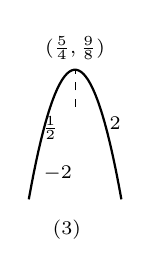
\begin{tikzpicture}[scale=0.42]
\ax{-1}{3.5}{-3}{2.2}
\draw[thick,domain=-0.15:2.65,samples=40] plot (\x,{-2*\x*\x+5*\x-2});
\draw[dashed] (1.25,0)--(1.25,1.125);
\node[right] at (0,-2){\scriptsize $-2$}; \node[above] at (1.25,1.125){\scriptsize $(\frac54,\frac98)$};
\node[below] at (0.5,0){\scriptsize $\frac12$}; \node[below right] at (2,0){\scriptsize 2};
\node at (1,-3.7){\scriptsize (3)};
\end{tikzpicture}